\documentclass[10pt,a4paper]{article}

\usepackage[utf8]{inputenc}
\usepackage{amsmath}
\usepackage{amsfonts}
\usepackage{amssymb}
\usepackage{tikz}
\usepackage{pgf}
\usetikzlibrary{arrows,automata}

\title{Implementation and evaluation of model checking using modal mu-calculus}

\author{Olav Bunte (0803961), Maurice Laveaux (0813568),\\ Ziad Ben Snaiba (0748095)}

\date{\today}

\begin{document}
\maketitle

\section{Introduction}

\section{Implementation}

\section{Implementation}

\subsection{Dining Philosophers}

\subsection{Demanding Children}

\subsection{Boardgame}

\section{Conclusion}


A picture of the labelled transition system.

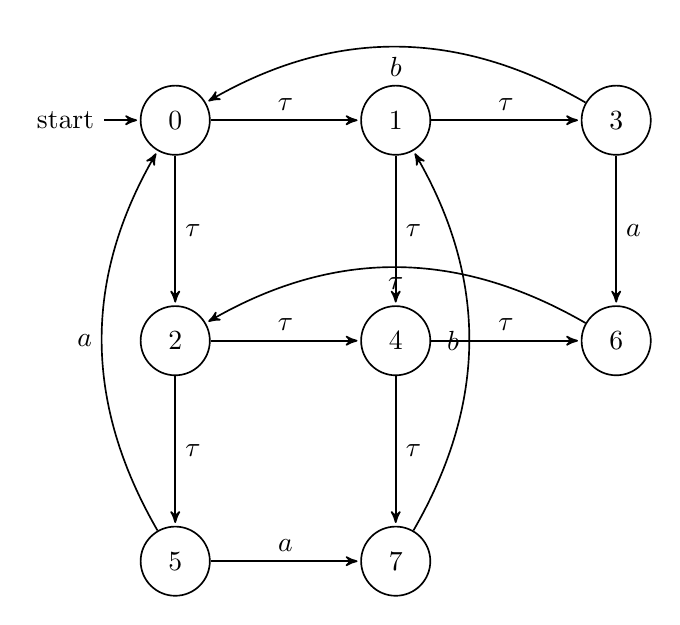
\begin{tikzpicture}[->,>=stealth', shorten >=1pt,auto, node distance=2.8cm, semithick]
  \tikzstyle{every state}=[text=black]

  \node[initial,state] (0)                    {$0$};
  \node[state]         (1) [right of=0] {$1$};
  \node[state]         (2) [below of=0] {$2$};
  \node[state]         (3) [right of=1] {$3$};
  \node[state]         (4) [below of=1] {$4$};
  \node[state]         (5) [below of=2] {$5$};
  \node[state]         (6) [right of=4] {$6$};
  \node[state]         (7) [below of=4] {$7$};
  
 \path (0) edge node {$\tau$} (1)
 	   (0) edge node {$\tau$} (2)
 	   (1) edge node {$\tau$} (3)
 	   (1) edge node {$\tau$} (4)
 	   (2) edge node {$\tau$} (5)
 	   (2) edge node {$\tau$} (4)
 	   (3) edge node {$a$} 	  (6)
 	   (3) edge [bend right] node {$b$} 	  (0)
 	   (4) edge node {$\tau$} (6)
 	   (4) edge node {$\tau$} (7)
 	   (5) edge [bend left] node {$a$}    (0)
 	   (5) edge node {$a$}    (7)
 	   (6) edge [bend right] node {$\tau$} (2)
 	   (7) edge [bend right] node {$b$}    (1);
\end{tikzpicture}

\end{document}